\chapter{\label{chap:simulation}Sistemas e Simulações}

``Simulação é a imitação da operação de um sistema ou processo do mundo real ao
longo do tempo.''~\cite{Banks}. Em outras palavras, simulação envolve a geração
de uma história artificial de um sistema ou processo e a observação desta
história de modo a obter inferências a respeito das características operacionais
da realidade ali representada. Para estudar tal sistema, frequentemente existe a
necessidade de realizar uma série de suposições sobre o seu funcionamento. Estas
suposições, que normalmente possuem a forma de relações matemáticas e lógicas,
constituem um modelo do sistema. Este modelo, por sua vez, é avaliado
numericamente enquanto são coletados dados de modo a tentar obter algum
entendimento sobre como o sistema correspondente se comporta.

Entretanto, existem diversas abordagens para se estudar e compreender um sistema
e suas características, dentre as quais a simulação. Entretanto, é senso comum
que cada sistema deve ser analisado através da ferramenta correta. Logo, embora
a simulação pareça ser uma boa alternativa à primeira vista, existe um extenso
conjunto de sistemas onde ela não é a forma mais apropriada para o seu estudo.
Assim, surge a importância métodos objetivos de verificar se a simulação é
apropriada para o caso estudado.

\section{\label{chap:waystostudy}Formas de Estudar um Sistema}

Ao realizar o estudo sobre um sistema e seu comportamento, uma gama de
estratégias podem ser colocadas em prática, dentre as quais podemos citar:
experimentar com o próprio sistema; experimentar com um modelo físico do
sistema; experimentar com um modelo matemático do sistema; etc. A fim de decidir
de forma objetiva qual a melhor abordagem para um dado sistema,~\cite{Law}
propõe esta reflexão através de 3 perguntas (figura~\ref{fig:systemstudy}). São
elas:

\begin{figure}[htb!]
\centering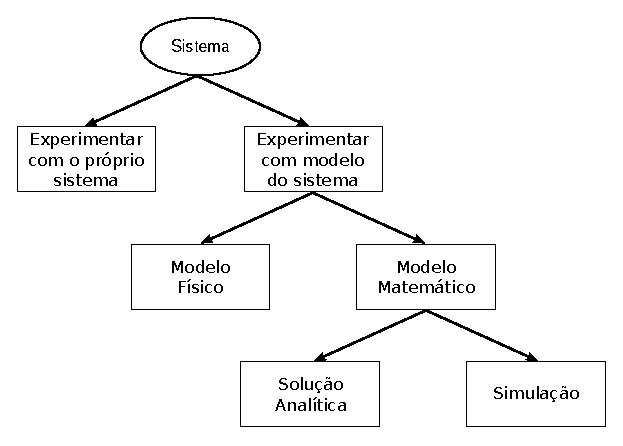
\includegraphics{img/systemstudy.eps}
\caption{\label{fig:systemstudy}Formas de estudar um sistema. Fonte:~\cite{Law}}
\end{figure}

\begin{enumerate}
\item \textit{Experimentar com o próprio sistema ou experimentar com um modelo do mesmo?}

Se houver viabilidade técnica e financeira na alteração de um sistema e na
observação de sua operação sob as novas condições, é desejável que se faça as
experimentações com o próprio sistema. Entretanto, frequentemente esta
alternativa é inviável por diversas razões:

\begin{itemize}
  \item O custo dos experimentos é muito elevado:

  % TODO - indentar no texto
  Exemplo: construir um novo módulo na Estação Espacial Internacional.

  \item O impacto causado pelos experimentos pode ser prejudicial ao sistema:

  % TODO - indentar no texto
  Exemplo: um mercado deseja reduzir o número de caixas a fim de diminuir seus
custos operacionais. Porém, esta medida pode causar um aumento significativo no
tamanho das filas - e consequentemente uma piora no tempo de espera dos clientes
e causar desistências.

  \item O sistema não existe:

  % TODO - indentar no texto
  Exemplo: o sistema ainda está nas fases de \textit{inception}, projeto ou
  desenvolvimento.
\end{itemize}

Por isto, muitas vezes é necessário realizar os experimentos utilizando um
\textit{modelo} como substituto ao sistema real. Entretanto, um sistema de
elevadores instalado e pronto para realizar as experimentações não encontra-se
entre os recursos disponíveis para a pesquisa neste estudo. Ainda, mesmo que tal
estrutura estivesse disponível, o número de cenários de testes possíveis seria
limitado pelas restrições físicas do sistema. Logo, optou-se pela utilização de
um modelo do sistema real.

\item \textit{Experimentar utilizando um modelo físico do sistema ou utilizar um modelo
matemático?}

Cockpits de aviões desacoplados do resto da nave, automóveis em escala em túneis
de vento e miniaturas funcioneis de sistemas de elevadores são alguns exemplos
de modelos físicos de sistemas. Ocasionalmente, este tipo de modelo é utilizado
é utilizado para estudar sistemas de engenharia ou logística~\cite{Law}.
Entretanto, a vasta maioria de modelos são matemáticos, representando um sistema
em termos de relações lógicas e quantitativas (equações matemáticas e notações
simbólicas), que são então manipuladas e alteradas para observar de que forma o
sistema real reagiria - isto se o modelo matemático for válido.

No contexto deste estudo, um modelo físico de um sistema de elevadores poderia
ser constituído pela maquete de um prédio com mini-elevadores movidos à motores
de passo - que por sua vez seriam controlados por microcontroladores.
Entretanto, este projeto por si só já seria grandioso demais - além de,
obviamente, fugir do escopo da Ciência da Computação e ser mais adequado à um
trabalho de conclusão de Engenharia Elétrica ou Engenharia de Controle e
Automação. Além disso, da mesma forma que em um sistema real de elevadores, o
número de cenários de testes seria limitado pelas restrições físicas do modelo
do sistema. Portanto, optou-se pela utilização de um modelo matemático do
sistema, reproduzível em ambiente computacional e facilmente parametrizável para
diferentes cenários.

\item \textit{O problema pode ser resolvido de forma analítica?}

De posse de um modelo matemático, o mesmo deve ser examinado de modo a verificar
de qual modo ele pode ser utilizado para dar solução ao problema que ele
representa. Segundo~\cite{Law}, se o modelo for simples o suficiente,
possivelmente é possível trabalhar com suas relações e equações para obter uma
solução exata, anaĺitica.~\cite{Law} cita como exemplo o modelo $d = vt$, onde
$d$ é a distância, $v$ é a velocidade média e $t$ é o tempo de viagem. Se
soubermos a distância a ser viajada e a velocidade, podemos trabalhar no modelo
e encontrar a equação $t = d/r$ para encontrar, exatamente, o tempo de viagem.
Embora esta solução seja simples, não é incomum a busca por soluções analíticas
tornar-se extraordinariamente complexa, exigindo vastos recursos computacionais.

Portanto, se uma solução analítica para um problema é conhecida e possui
eficiência computacional, é mais apropriado estudar este sistema desta forma do
que através de simulação. Do contrário, o sistema deve ser estudado através de
simulações~-~ou~seja, exercitar numericamente as entradas do modelo matemático
do sistema e observar de que forma estes exercícios afetam as saídas.
Entretanto, conforme afirmado no capítulo \ref{chap:intro} deste estudo, o
problema de atribuir elevadores para atender chamadas feitas pelos passageiros
minimizando alguma métrica encontra-se no conjunto de problemas NP- difícil (ou
NP-hard, ou NP-complexo)~\cite{SeKo99}. Assim, uma solução ótima, computável em
tempo polinomial, ainda não é conhecida para este problema. Logo, o problema não
pode ser resolvido de forma anaĺitica. Este fato vai ao encontro dos grandes
esforços da indústria em procurar soluções para resolver o problema ao longo das
décadas, não poupando esforços e investimentos em busca desta solução.

\end{enumerate}

Em outra abordagem,~\cite{BanksGibson} define 10 situações onde a simulação
\textbf{não} é indicada. Tais situações são:

\begin{enumerate}
\item \textit{Quando o problema puder ser resolvido utilizando-se de bom senso}

Conforme discutido anteriormente neste capítulo, dada a complexidade do problema
(NP-completo), não é possível encontrar a solução apenas utilizando o bom senso.

\item \textit{Quando o problema puder ser resolvido de forma analítica}

Ainda sobre a complexidade NP-completo, este fato implica no desconhecimento de
uma forma analítica para encontrar a sua solução.

\item \textit{Quando o problema puder ser resolvido através de experimentos
diretamente no sistema}

Como já constatado, não há um sistema de elevadores instalado para realizar as
experimentações entre os recursos disponíveis para este estudo. E, mesmo que
houvesse, haveria um limite nos cenários de testes em função das restrições
físicas do sistema. Logo, não é possível realizar experimentos diretamente no
sistema.

\item \textit{Quando seus custos da simulação excederem os seus ganhos}

Embora os custos de modelagem, projeto e implementação do simulador deste estudo
não tenham sido avaliados de forma direta, acredita-se que os resultados trarão
benefícios aos usuários de elevadores, conforme explicitado nos capítulos
\ref{chap:intro}, \ref{chap:problem} e \ref{chap:proposal} deste estudo.

\item \textit{Quando não há recursos financeiros suficientes}

TO-DO % TO-DO

\item \textit{Quando não há tempo suficiente}

TO-DO % TO-DO

\item \textit{Quando não há dados suficientes, nem mesmo estimativas}

TO-DO % TO-DO

\item \textit{Quando não há possibilidade de verificar a validade do modelo}

TO-DO % TO-DO

\item \textit{Quando as expectativas e o poder da simulação são superestimados}

Neste estudo o foco das expectativas está nos ganhos que a Inteligência
Artificial pode trazer para estes sistemas. A simulação é vista apenas como uma
forma para avaliar os resultados obtidos. Portanto, a simulação não é
superestimada e o caso não se enquadra nesta situação.

\item \textit{Quando o comportamento do sistema é muito complexo ou não pode ser
definido (e.~g. seres humanos)}

Um \textbf{EGCS} não é um sistema de alta complexidade, possuindo um conjunto de
comportamentos limitado e um espaço de estados finito. Portanto, não se enquadra
nesta situação.

\end{enumerate}

Em função destas reflexões justifica-se a simulação como uma forma apropriada
para estudar um \textbf{EGCS}.

\section{Classificação do Modelo de Simulação}

De posse de um modelo matemático a ser estudado por meio de simulação (doravante
chamado de \textit{modelo de simulação}), o mesmo pode ser classificado em três
dimensões~\cite{Banks,Law}:

\begin{enumerate}
\item Estático ou Dinâmico

Um modelo de simulação estático é uma representação de um sistema em um ponto
particular no tempo, ou então um sistema onde o tempo simplesmente é
irrelevante. Por outro lado, um modelo de simulação dinâmico representa um
sistema que evolui e se modifica com o passar do tempo.

No escopo deste trabalho, o modelo de simulação é claramento dinâmico. Deseja-se
verificar o comportamento do sistema ao longo de um intervalo de tempo finito,
na medida em que passageiros chegam e elevadores os transportam através dos
andares do prédio.

\item Determinístico ou Estocástico

Um modelo de simulação que não possua nenhum componente probabilístico (i.~e,~
aleatoriedade) é chamado de \textit{determinístico}. Em um modelo de simulação
\textit{determinístico} sua saída é ``determinada'' no momento em que a sua
entrada é definida - mesmo que ainda tome tempo computacional para realizar o
cálculo de qual seja o resultado \cite{Law}. Em outras palavras, significa dizer
que a saída fornecida pelo modelo de simulação será sempre a mesma para uma
mesma entrada. Porém a grande maioria dos sistemas do mundo real possuem, no
mínimo, algum grau de aleatoridade na sua entrada. Estes sistemas dão origem a
modelos de simulação \textit{estocásticos}. Estes, diferentemente de modelos
\textit{determinísticos}, fornecem uma saída igualmente aleatória~-~e, por esta
razão, esta saída deve ser considerada como um conjunto de \textit{estimativas}
das características reais do sistema, e não as características propriamente
ditas \cite{Banks}.

Em um \textbf{EGCS} real não é possível prever quantos passageiros utilizarão o
sistema, quando eles chegarão e tampouco para qual andar irão. Portanto, um
modelo de simulação válido neste escopo deve ser \textit{estocástico} de modo a
lidar com a aleatoridade da entrada de passageiros no sistema.

\item Contínuo ou Discreto

A figura \ref{fig:disccont} ilustra o comportamento de uma variável de estado em
modelos de simulação \textit{contínuos} e \textit{discretos}. O modelo
\textit{contínuo} é aquele onde os valores das variáveis mudam continuamente ao
longo do tempo. Já em um modelo \textit{discreto} as variáveis de estado teu sem
valor alterado instantaneamente em determinados instantes separados do tempo
\cite{Banks}. É importante salientar que modelos discretos não necessariamente
representam sistemas discretos e vice-versa \cite{Law}. A decisão por um modelo
ou outro se dá especificamente pelos objetivos do estudo.

Para este projeto, não há a necessidade - tampouco a disposição de tempo
computacional - de informações instantâneas a respeito da movimentação de
passageiros e elevadores, e sim de observar o comportamento do sistema dada a
ocorrência de determinados eventos, e.~g., um passageiro embarca em um elevador.
Portanto, no escopo deste estudo utilizaremos um modelo de simulação
\textit{discreto}.

\begin{figure}[htb!]
\centering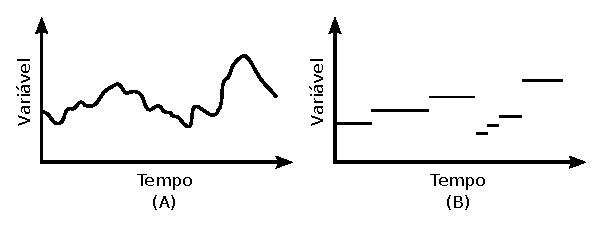
\includegraphics{img/discrete_continuous.eps}
\caption{\label{fig:disccont}Variável de estado em um modelo contínuo (A) e discreto (B). Fonte:~\cite{Banks}}
\end{figure}

\end{enumerate}

Portanto, será utilizado um modelo de simulação \textit{dinâmico},
\textit{estocástico} e \textit{discreto} para representar um \textbf{EGCS}.

\section{Simulação de Eventos Discretos com Avanço de Tempo}

Conceitos \cite{Banks}:

\begin{description}
\item[Sistema] TO-DO % TO-DO
\item[Modelo] TO-DO % TO-DO
\item[Estado do Sistema] TO-DO % TO-DO
\item[Entidade] TO-DO % TO-DO
\item[Atributo] TO-DO % TO-DO
\item[Lista] TO-DO % TO-DO
\item[Evento] TO-DO % TO-DO
\item[Notificação de Evento] TO-DO % TO-DO
\item[Lista de Eventos] TO-DO % TO-DO
\item[Atividade] TO-DO % TO-DO
\item[Atraso] TO-DO % TO-DO
\item[Relógio] TO-DO % TO-DO
\end{description}

\subsection{Mecanismo de Avanço de Tempo}

\subsection{Componentes de um Modelo de Simulação de Eventos Discretos}